\documentclass[10pt,a4paper]{article}

\usepackage[margin=18mm]{geometry}

\usepackage[T1]{fontenc}

\usepackage{lmodern,booktabs,longtable,graphicx,pdflscape,hyperref}

\hypersetup{colorlinks=true,urlcolor=blue}

\setlength{\parindent}{0pt}

\setlength{\parskip}{5pt}

\setlength{\emergencystretch}{2em}

\begin{document}

\begin{center}{\Large\bfseries Equal-total-time PointSAT study}\end{center}

\section*{Method and endpoint}

Each registered SAT target and native seed is compared under a single total-wall-time allowance. Runtime preparation and imports, flippability, native search, SAT feedback, and online verification all share the same clock. Initial SAT target sampling is outside this clock and reported separately as corpus construction. No state is shared between treatment arms or targets.

This is a cold realization-workflow comparison, not the literal untouched PointSAT driver or steady-state batch throughput. The original arm uses the frozen original flippability implementation and untouched native solver. Updated arms use the revised checker, persistent only within one trajectory. Conversion, the required compressed-variable adapter, storage and geometric acceptance are common. Original-to-updated continuous changes both preparation and the native package; updated plain/line/pair comparisons isolate native flags. Cold preparation may dominate short allowances, especially for 19 points.

The primary event is the first accepted solution returned by completed online verification before the deadline. We use logged verification-completion timestamps tied to immutable checked certificates, not estimated native discovery times. A posthoc-valid coordinate file cannot create or backdate an online success. For 19 points, numeric geometric validity is distinct from exact threefold-symmetry reconstruction; the latter is a secondary posthoc claim. Actual x-direction caps are checked for the cap family.

Continuous arms and segmented arms have intentionally different candidate-return opportunities. Retry-only controls use the segmented schedule without SAT feedback. Their comparison measures the additional feedback workflow under the same total allowance, not a fixed-work native-kernel speedup.

All registered targets remain in empirical verified-return denominators. Failures have no success event and retain censor times. This is a small, deliberately diverse, non-IID corpus with one native seed per target; no universal success rate or speed multiplier is established. The curves are actual step functions, not interpolated time-to-discovery estimates.

\textbf{Protocol correction.} Earlier native-only-budget runs remain separate partial diagnostics. Their outcomes, costs, or native seconds are not converted into equal-total-time observations. The same fixed targets are reused after those diagnostics; this is not an unseen holdout evaluation.

\section*{Verified returns by total wall time}

Cells show verified returns / all registered targets. The parenthetical U count identifies targets neither observed through that milestone nor already solved; those targets are not removed from the denominator.

\begin{center}\small\begin{longtable}{llrrr}
\toprule
Problem & Arm & 30 s & 60 s & 120 s \\
\midrule\endhead
symmetry19 & Upstream & 0/20 (U0) & 0/20 (U0) & 0/20 (U0) \\
symmetry19 & v4 continuous & 0/20 (U0) & 0/20 (U0) & 0/20 (U0) \\
symmetry19 & v4 retry only & 0/20 (U0) & 0/20 (U0) & 1/20 (U0) \\
symmetry19 & v4 SAT feedback & 0/20 (U0) & 1/20 (U0) & 2/20 (U0) \\
gons32 & Upstream & 0/20 (U0) & 0/20 (U0) & 0/20 (U0) \\
gons32 & v6 plain & 0/20 (U0) & 0/20 (U0) & 0/20 (U0) \\
gons32 & v6 line & 0/20 (U0) & 0/20 (U0) & 0/20 (U0) \\
gons32 & v6 line+pair & 0/20 (U0) & 0/20 (U0) & 0/20 (U0) \\
gons32 & v6 retry only & 0/20 (U0) & 0/20 (U0) & 0/20 (U0) \\
gons32 & v6 SAT feedback & 0/20 (U0) & 0/20 (U0) & 0/20 (U0) \\
caps26 & Upstream & 0/20 (U0) & 0/20 (U0) & 0/20 (U0) \\
caps26 & v6 plain & 0/20 (U0) & 0/20 (U0) & 0/20 (U0) \\
caps26 & v6 line & 0/20 (U0) & 0/20 (U0) & 0/20 (U0) \\
caps26 & v6 line+pair & 0/20 (U0) & 0/20 (U0) & 0/20 (U0) \\
caps26 & v6 retry only & 0/20 (U0) & 0/20 (U0) & 0/20 (U0) \\
caps26 & v6 SAT feedback & 0/20 (U0) & 0/20 (U0) & 0/20 (U0) \\
holes29 & Upstream & 0/20 (U0) & 0/20 (U0) & 0/20 (U0) \\
holes29 & v6 plain & 0/20 (U0) & 0/20 (U0) & 0/20 (U0) \\
holes29 & v6 line & 0/20 (U0) & 0/20 (U0) & 0/20 (U0) \\
holes29 & v6 line+pair & 0/20 (U0) & 0/20 (U0) & 0/20 (U0) \\
holes29 & v6 retry only & 0/20 (U0) & 0/20 (U0) & 0/20 (U0) \\
holes29 & v6 SAT feedback & 0/20 (U0) & 5/20 (U0) & 12/20 (U0) \\
mixed23 & Upstream & 0/20 (U0) & 0/20 (U0) & 0/20 (U0) \\
mixed23 & v6 plain & 0/20 (U0) & 0/20 (U0) & 0/20 (U0) \\
mixed23 & v6 line & 0/20 (U0) & 0/20 (U0) & 0/20 (U0) \\
mixed23 & v6 line+pair & 0/20 (U0) & 0/20 (U0) & 0/20 (U0) \\
mixed23 & v6 retry only & 0/20 (U0) & 0/20 (U0) & 0/20 (U0) \\
mixed23 & v6 SAT feedback & 0/20 (U0) & 4/20 (U0) & 4/20 (U0) \\
\bottomrule\end{longtable}\end{center}


\clearpage\begin{landscape}

\section*{Actual first-verified-return curves}

\begin{center}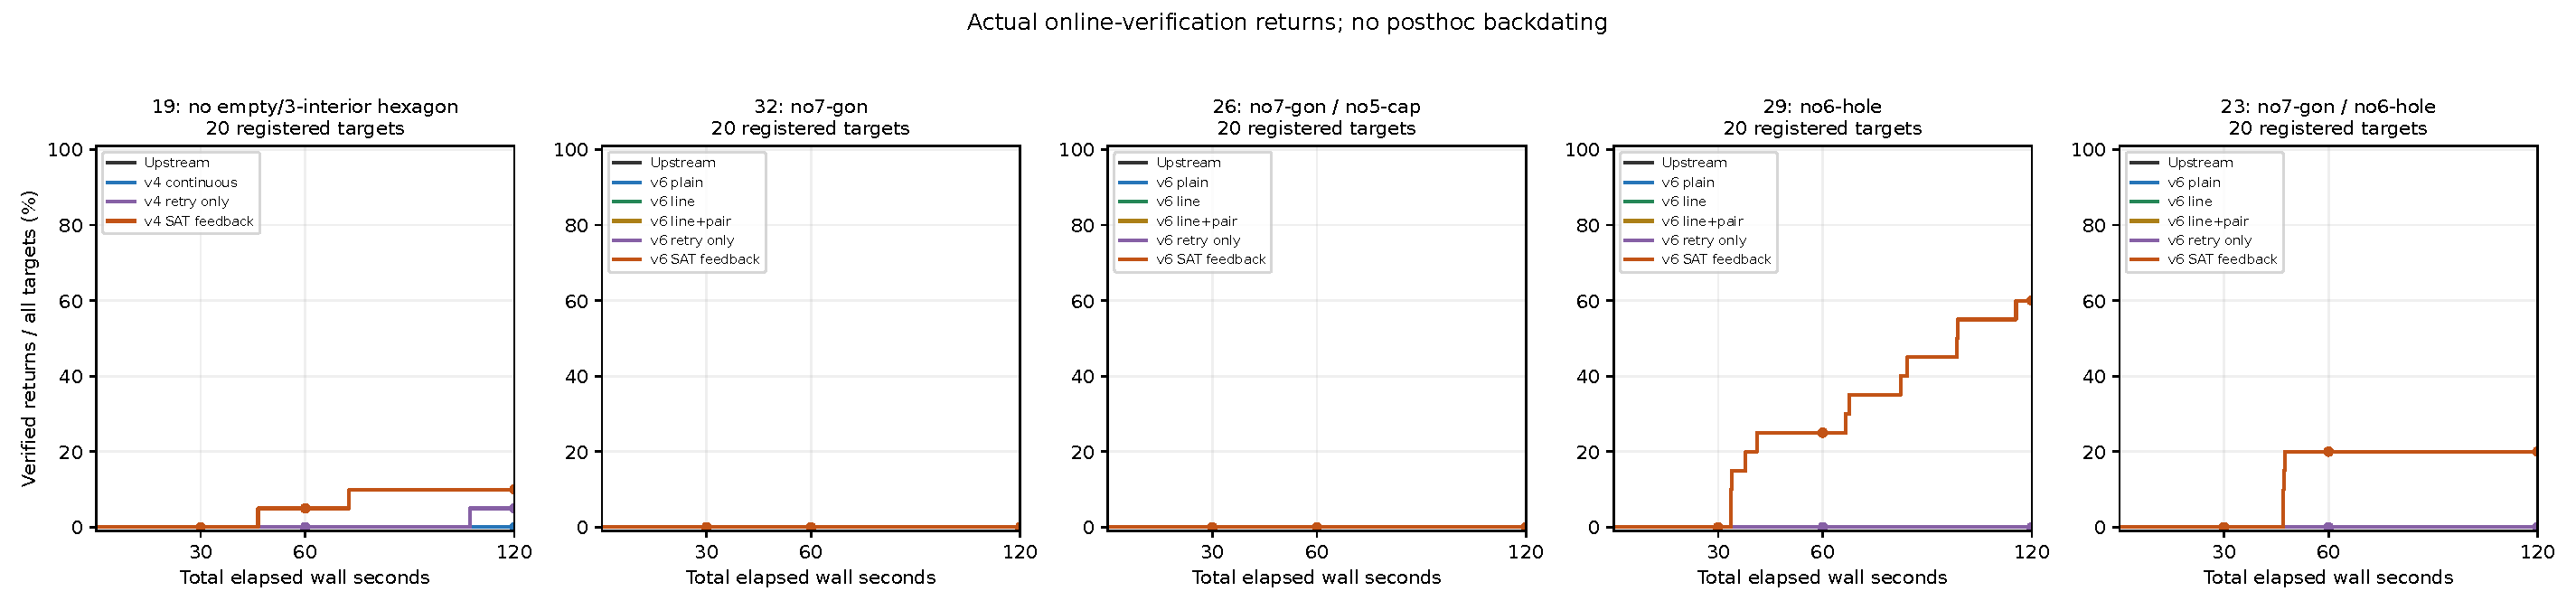
\includegraphics[width=\linewidth,height=100mm,keepaspectratio]{verified-returns.pdf}\end{center}

Every event occurs at its recorded verification-completed elapsed time. Hollow milestone markers indicate incomplete exposure. Failures remain censored rather than being assigned invented success times. Coincident arm values can overlap. This is the empirical fraction of all registered targets, not a Kaplan--Meier extrapolation.

\end{landscape}\clearpage

\section*{Matched retry-only versus SAT-feedback outcomes}

All target identities are paired. A first-only result favors retry-only; a second-only result favors feedback. Both and neither are retained; provisional pairs have incomplete exposure. All other arm pairs, including upstream comparisons, are in README.md/report.json.

\begin{center}\small\begin{longtable}{lrrrrrr}
\toprule
Problem & Wall s & Retry only & Feedback only & Both & Neither & Provisional \\
\midrule\endhead
symmetry19 & 30 & 0 & 0 & 0 & 20 & 0 \\
symmetry19 & 60 & 0 & 1 & 0 & 19 & 0 \\
symmetry19 & 120 & 0 & 1 & 1 & 18 & 0 \\
gons32 & 30 & 0 & 0 & 0 & 20 & 0 \\
gons32 & 60 & 0 & 0 & 0 & 20 & 0 \\
gons32 & 120 & 0 & 0 & 0 & 20 & 0 \\
caps26 & 30 & 0 & 0 & 0 & 20 & 0 \\
caps26 & 60 & 0 & 0 & 0 & 20 & 0 \\
caps26 & 120 & 0 & 0 & 0 & 20 & 0 \\
holes29 & 30 & 0 & 0 & 0 & 20 & 0 \\
holes29 & 60 & 0 & 5 & 0 & 15 & 0 \\
holes29 & 120 & 0 & 12 & 0 & 8 & 0 \\
mixed23 & 30 & 0 & 0 & 0 & 20 & 0 \\
mixed23 & 60 & 0 & 4 & 0 & 16 & 0 \\
mixed23 & 120 & 0 & 4 & 0 & 16 & 0 \\
\bottomrule\end{longtable}\end{center}


\section*{Compute accounting}

All recorded attempts contribute, including failed and interrupted work. CPU seconds measure processor consumption; wall is never substituted for missing CPU. Parent totals overlap component costs and must not be added to them. Summed worker wall is not elapsed calendar duration. Posthoc audit costs are outside the primary clock. No cost average is conditioned only on successful trials.

\begin{center}\small\begin{longtable}{llrrrr}
\toprule
Problem & Arm & Prep CPU s & Native CPU s & Feedback CPU s & Online check CPU s \\
\midrule\endhead
symmetry19 & Upstream & 325.64 & 2003.36 & -- & 0.43 \\
symmetry19 & v4 continuous & 364.14 & 1966.37 & -- & 0.48 \\
symmetry19 & v4 retry only & 363.56 & 1949.89 & -- & 3.37 \\
symmetry19 & v4 SAT feedback & 364.26 & 1118.61 & 757.43 & 1.89 \\
gons32 & Upstream & 111.55 & 2219.61 & -- & 29.43 \\
gons32 & v6 plain & 16.36 & 2315.49 & -- & 43.38 \\
gons32 & v6 line & 16.16 & 2313.68 & -- & 40.24 \\
gons32 & v6 line+pair & 16.25 & 2317.13 & -- & 40.32 \\
gons32 & v6 retry only & 16.31 & 2033.20 & -- & 322.41 \\
gons32 & v6 SAT feedback & 16.29 & 1999.05 & 48.33 & 305.52 \\
caps26 & Upstream & 28.36 & 2304.05 & -- & 0.05 \\
caps26 & v6 plain & 7.66 & 2324.44 & -- & 0.05 \\
caps26 & v6 line & 7.65 & 2322.41 & -- & 0.05 \\
caps26 & v6 line+pair & 7.61 & 2324.90 & -- & 0.06 \\
caps26 & v6 retry only & 7.71 & 2320.93 & -- & 0.41 \\
caps26 & v6 SAT feedback & 7.62 & 2270.75 & 26.82 & 0.61 \\
holes29 & Upstream & 102.18 & 2230.53 & -- & 3.57 \\
holes29 & v6 plain & 39.79 & 2291.78 & -- & 6.18 \\
holes29 & v6 line & 39.64 & 2292.75 & -- & 6.32 \\
holes29 & v6 line+pair & 40.05 & 2290.00 & -- & 6.47 \\
holes29 & v6 retry only & 40.06 & 2238.88 & -- & 55.08 \\
holes29 & v6 SAT feedback & 39.58 & 1552.80 & 89.25 & 38.53 \\
mixed23 & Upstream & 26.71 & 2306.48 & -- & 3.06 \\
mixed23 & v6 plain & 19.03 & 2314.23 & -- & 5.01 \\
mixed23 & v6 line & 19.07 & 2311.28 & -- & 5.34 \\
mixed23 & v6 line+pair & 19.06 & 2312.75 & -- & 4.74 \\
mixed23 & v6 retry only & 19.07 & 2273.43 & -- & 39.94 \\
mixed23 & v6 SAT feedback & 19.12 & 1977.05 & 21.00 & 36.27 \\
\bottomrule\end{longtable}\end{center}


\begin{center}\small\begin{longtable}{rrrrrr}
\toprule
Study & Attempts & Parent CPU s & Parent wall s & Posthoc CPU s & Posthoc wall s \\
\midrule\endhead
1 & 560 & 64684.84 & 66336.41 & 445.44 & 456.43 \\
\bottomrule\end{longtable}\end{center}


\section*{Censoring, errors and provenance}

Registered trajectories: 560; completed: 560; persisted attempts: 560; incomplete: 0; repeat attempts: 0; late verification events excluded: 0. Statuses: \{"SOLVED": 19, "TIME\_LIMIT": 541\}.

Online deadline-exceeded checks: 9; online checker errors: 0; search CPU lower-bound attempts: 424; posthoc CPU lower-bound attempts: 0. Abruptly killed descendants may leave unrecorded CPU, so affected totals are lower bounds rather than complete exact measurements.

Corpus strata: \{"fresh": 9, "historical\_initial\_sat": 11\}. Fresh SAT generation and reused historical/proof-filtered targets are distinct strata. Historical selection used initial SAT assignments in fixed source order, not coordinate or feedback outcomes. The known positive-control canonical type is excluded. Generation-only cuts do not enter the benchmark original CNF.

Outside-clock corpus construction: 1798.74 fresh-generation CPU seconds; 12.54 combined-corpus revalidation CPU seconds. These are separate timers; historical generation sunk costs are not attributed to this batch.

{\small Registration: \url{/home/andrew/PointSAT/benchmarks/anytime_20260907/registration.json}}\\{\footnotesize\texttt{bc9b176c5c291e62660c29a78155b06943a0a5f9d92cd754158a429cc9812f58}}

An operational error or a deadline without a returned solution is not an impossibility proof. The JSON retains each censor timestamp, certificate hash, all arm pairs, component timing coverage, and every recorded error. A duplicate completed case/arm is an integrity failure rather than an opportunity to pick the better run.

\section*{Separate earlier positive control}

The supplied control file belongs to a known realizable target excluded from the main diverse corpus. It is an earlier pipeline sanity check, not an additional equal-total-time trial. Its native timings are not first-verified-return times and are not pooled into these curves.

{\small\url{/home/andrew/PointSAT/benchmarks/compare19_positive_control_20260907/result.json}}

Machine/environment snapshot: {\small\url{/home/andrew/PointSAT/benchmarks/scaling_machine_20260907.json}}. The recorded environment is virtualized; its reported CPU model and visible logical topology do not establish dedicated physical cores. The study has a two-worker budget; measured CPU and wall costs are retained separately.

This report was generated read-only from the new equal-total-time registration and committed SQLite records. No native search or geometry audit runs during reporting. README.md and report.json accompany this PDF, together with its LaTeX source and vector/PNG figure. All earlier reports are preserved.

\end{document}

